\documentclass[a4paper]{jsarticle}
\usepackage{amsmath,amssymb,bm}
\usepackage{graphicx}
\usepackage{ascmac}
\everymath{\displaystyle}

\flushbottom
\sloppy

\setlength{\paperwidth}{210mm}
\setlength{\hoffset}{0mm}
\setlength{\textwidth}{\paperwidth}
\addtolength{\textwidth}{-30mm}
\setlength{\oddsidemargin}{-1in}
\addtolength{\oddsidemargin}{15mm}
\setlength{\columnsep}{7mm}

\setlength{\paperheight}{297mm}
\setlength{\voffset}{0mm}
\setlength{\textheight}{\paperheight}
\addtolength{\textheight}{-60mm}
\setlength{\topmargin}{-1in}
\addtolength{\topmargin}{20mm}
\setlength{\headheight}{0mm}
\setlength{\headsep}{0mm}
\setlength{\footskip}{10mm}

\title{線形計画法(2段階単体法)}

\begin{document}
\maketitle

線形計画法は最適化の例として分かりやすくかつ実用例も多いので,
解説は数多く存在しますが,
退化や過剰制約のケースまでカバーしたものがあまり見られないので自分で書いてみました.
なお,本記事の作成にあたって主に次の書籍を参考にしました.

岩波講座応用数学[方法7] 最適化法,藤田 宏,今野 浩,田邉 國士著,岩波書店,1994

\section{線形計画問題の標準形}

線形計画問題とは,
ある線形方程式$\boldsymbol{A}\boldsymbol{x}=\boldsymbol{b}$を満たす$\boldsymbol{x}$のうち,
ある線形関数$z=\boldsymbol{c}^{\mathrm{T}}\boldsymbol{x}$の値を最小化する
$\boldsymbol{x}=\boldsymbol{x}^{*}$を求める問題です.
\begin{align}
\begin{array}{c}
\boldsymbol{x}^{*}=\mathop{\mathrm{arg~min}}_{\boldsymbol{x}}\left\{\boldsymbol{c}^{\mathrm{T}}\boldsymbol{x}
\left|\boldsymbol{x}\in\mathcal{X}\right.
\right\}
\\
\mathcal{X}=\left\{\boldsymbol{x}\left|
\boldsymbol{A}\boldsymbol{x}=\boldsymbol{b},
\boldsymbol{x}\geq\boldsymbol{0}
\right.
\right\}
\end{array}
\label{pb:lp}
\end{align}
$\boldsymbol{x}$は{\bf 設計変数},
$\boldsymbol{x}^{*}$は{\bf 最適解},
$z$は{\bf 目的関数}(あるいは{\bf 評価関数},{\bf 損失関数})などと呼ばれます.
$\mathcal{X}$の元$\boldsymbol{x}$が満たす条件に$\boldsymbol{x}\geq\boldsymbol{0}$が加えられていますが,
これは便宜上のものです.
もし$\boldsymbol{x}$が負になっても構わないならば,
二つの非負変数ベクトル$\boldsymbol{x}_{+}$および$\boldsymbol{x}_{-}$を用いて
$\boldsymbol{x}=\boldsymbol{x}_{+}-\boldsymbol{x}_{-}$とおくことで,元の方程式を
\begin{align*}
\begin{bmatrix}
\boldsymbol{A} & -\boldsymbol{A}
\end{bmatrix}
\begin{bmatrix}
\boldsymbol{x}_{+} \\ \boldsymbol{x}_{-}
\end{bmatrix}
=
\boldsymbol{b},\qquad
\begin{bmatrix}
\boldsymbol{x}_{+} \\ \boldsymbol{x}_{-}
\end{bmatrix}
\geq\boldsymbol{0}
\end{align*}
と表せます.
また,$\boldsymbol{x}$が満たすべき条件が線形方程式ではなく線形不等式$\boldsymbol{Ax}\leq\boldsymbol{b}$である場合には,
非負変数ベクトル$\boldsymbol{x}^{\prime}$を新たに設計変数に追加することで
\begin{align*}
\begin{bmatrix}
\boldsymbol{A} & \boldsymbol{1}
\end{bmatrix}
\begin{bmatrix}
\boldsymbol{x} \\ \boldsymbol{x}^{\prime}
\end{bmatrix}
=
\boldsymbol{b},\qquad
\begin{bmatrix}
\boldsymbol{x} \\ \boldsymbol{x}^{\prime}
\end{bmatrix}
\geq\boldsymbol{0}
\end{align*}
のように線形方程式に置き換えられます(ただし$\boldsymbol{1}$は単位行列).
このとき追加した$\boldsymbol{x}^{\prime}$は{\bf スラック変数}と呼ばれます.
いずれの場合でも,
拡張された変数およびその係数行列を改めて$\boldsymbol{x}$,$\boldsymbol{A}$とそれぞれおき直せば,
問題(\ref{pb:lp})の形に帰着します.
この意味で問題(\ref{pb:lp})の定式化には一般性があり,
{\bf 線形計画問題の標準形}と呼ばれます.

\begin{figure}[h]
\begin{center}
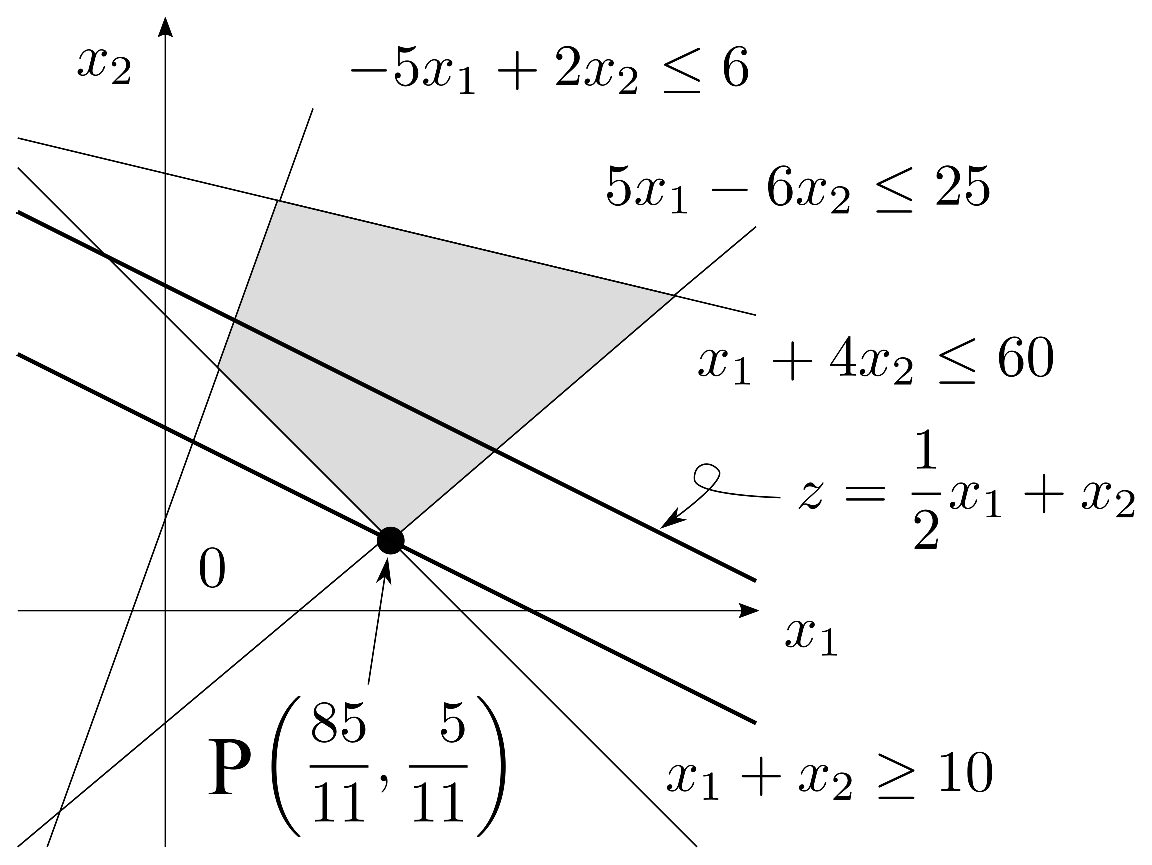
\includegraphics[width=.4\textwidth]{fig/LP_feasibleregion.eps}
\caption{線形計画問題の例}
\label{fig:LP_feasibleregion}
\end{center}
\end{figure}

例えば次の4つの不等式
\begin{align*}
x_{1}+x_{2} &\geq 10
\\
x_{1}+4x_{2} &\leq 60
\\
5x_{1}-6x_{2} &\leq 25
\\
-5x_{1}+2x_{2} &\leq 6
\end{align*}
で表される領域は,
図\ref{fig:LP_feasibleregion}の灰色い四角形の内部および縁上となりますが,
これは次のようにも表せます.
\begin{align*}
\begin{bmatrix}
-1 & -1 & 1 & 0 & 0 & 0 \\
 1 &  4 & 0 & 1 & 0 & 0 \\
 5 & -6 & 0 & 0 & 1 & 0 \\
-5 &  2 & 0 & 0 & 0 & 1 \\
\end{bmatrix}
\begin{bmatrix}
x_{1} \\ x_{2} \\ x_{3} \\ x_{4} \\ x_{5} \\ x_{6}
\end{bmatrix}
=
\begin{bmatrix}
-10
\\
60
\\
25
\\
6
\end{bmatrix}
,\qquad
\begin{bmatrix}
x_{1} \\ x_{2} \\ x_{3} \\ x_{4} \\ x_{5} \\ x_{6}
\end{bmatrix}
\geq
\begin{bmatrix}
0 \\ 0 \\ 0 \\ 0 \\ 0 \\ 0
\end{bmatrix}
\end{align*}
この下で例えば
\begin{align*}
z=\frac{1}{2}x_{1}+x_{2}
=\begin{bmatrix}
\frac{1}{2} & 1 & 0 & 0 & 0 & 0
\end{bmatrix}
\begin{bmatrix}
x_{1} \\ x_{2} \\ x_{3} \\ x_{4} \\ x_{5} \\ x_{6}
\end{bmatrix}
\end{align*}
を最小化したいとしましょう.
$z$は図中の太い直線の$x_{2}$軸切片ですから,
この直線を灰色領域と交わる範囲でできるだけ下方に動かしたい,
という要求と解釈できます.
そしてこの要求は,この直線が点P$(85/11, 25/11)$を通るときに満たされるとすぐに分かります.
つまり最適解は$[x_{1}^{*}~x_{2}^{*}~x_{3}^{*}~x_{4}^{*}~x_{5}^{*}~x_{6}^{*}]^{\mathrm{T}}=[85/11~25/11~0~\bullet~0~\bullet]^{\mathrm{T}}$で,
対応する$z$の最小値は$135/22$です
($\bullet$には対応するスラック変数の値が入りますが,
元々知りたかったのは$x_{1}$,$x_{2}$だけなので省略します).

\section{単体法}

\subsection{基本的な考え方}

線形計画問題の解法(線形計画法)は幾つかありますが,
単体法は最も簡単な,かつ設計変数の数が数百程度までならば十分に実用的な方法と言われています.
上図のように,
$\mathcal{X}$で表される領域は超多角形をなし,
最適解はその頂点のどれかになると考えられるので,
それらの頂点のうち目的関数の値を最小にするものを探す,
というのが基本的な考え方です.
全ての頂点について目的関数を調べていては効率が悪いので,
隣接する頂点のうち目的関数を減らすものだけを選んで辿っていく,
という巧妙な方法がとられます.

前提として$\mathcal{X}$が空集合でないためには,
$\boldsymbol{A}$のランクが設計変数の数($\mathcal{X}$の次元)以下であることが必要条件となります.
$\boldsymbol{A}$が$m\times n$行列で,
かつ行フルランクであるならば,
この条件は$m\leq n$と同値です.
一般的には,
$m\leq n$であっても$\boldsymbol{A}$が行フルランクであるとは限らないし,
$\mathcal{X}$が空集合でないかどうかもすぐには分からないのですが,
これらのことは後で考えることにしましょう.

以下,$\boldsymbol{A}$,$\boldsymbol{b}$,$\boldsymbol{c}$それぞれの成分を
\begin{align*}
\boldsymbol{A}=\begin{bmatrix}
\boldsymbol{a}_{1} & \cdots & \boldsymbol{a}_{n}
\end{bmatrix}=\begin{bmatrix}
a_{11} & \hdots & a_{1n} \\
\vdots & \ddots & \vdots \\
a_{m1} & \hdots & a_{mn}
\end{bmatrix},
\quad
\boldsymbol{b}=\begin{bmatrix}
b_{1} \\ \vdots \\ b_{m}
\end{bmatrix},
\quad
\boldsymbol{c}=\begin{bmatrix}
c_{1} \\ \vdots \\ c_{n}
\end{bmatrix}
\end{align*}
と表すことにします.
$n$個ある設計変数のうち$m$個を適当に選んで,
それらの添字の集合を$\mathcal{J}_{\mathrm{B}}=\left\{j_{\mathrm{B}1},\cdots,j_{\mathrm{B}m}\right\}$,
残りの添字の集合を$\mathcal{J}_{\mathrm{N}}=\left\{j_{\mathrm{N}1},\cdots,j_{\mathrm{N}n-m}\right\}$とそれぞれおきましょう.
このとき
\begin{align}
\boldsymbol{A}\boldsymbol{x}&\equiv
 \sum_{k=1}^{m}\boldsymbol{a}_{j_{\mathrm{B}k}}x_{j_{\mathrm{B}k}}
+\sum_{k=1}^{n-m}\boldsymbol{a}_{j_{\mathrm{N}k}}x_{j_{\mathrm{N}k}}
\left(=\boldsymbol{b}\right)
\label{eq:lp_eq_pivot}
\\
\boldsymbol{c}^{\mathrm{T}}\boldsymbol{x}&\equiv
 \sum_{k=1}^{m}c_{j_{\mathrm{B}k}}x_{j_{\mathrm{B}k}}
+\sum_{k=1}^{n-m}c_{j_{\mathrm{N}k}}x_{j_{\mathrm{N}k}}
\left(=z\right)
\label{eq:lp_eq_cost}
\end{align}
のように,方程式と目的関数を二つの添字グループそれぞれの寄与分に分けて考えることができます.
$\boldsymbol{a}_{j_{\mathrm{B}k}}$($k=1,\cdots,m$)が全て互いに線形独立であるとき,
$\mathcal{J}_{\mathrm{B}}$で表される設計変数のグループを{\bf 基底}と呼びます.
これに対し
$\mathcal{J}_{\mathrm{N}}$で表される設計変数のグループを{\bf 非基底}と呼びます.

ここで,次のような特殊な状況を考えます.
\begin{screen}
\begin{itemize}
\item{全ての$\boldsymbol{a}_{j_{\mathrm{B}k}}$($k=1,\cdots,m$)が,$k$番目成分だけ$1$で残り全て$0$のベクトルである.}
\item{全ての$c_{j_{\mathrm{B}k}}$($k=1,\cdots,m$)が$0$である.}
\end{itemize}
\end{screen}
つまり,
\begin{align*}
\begin{bmatrix}
x_{j_{\mathrm{B}1}} \\
\vdots \\
x_{j_{\mathrm{B}m}} \\
\end{bmatrix}+\sum_{k=1}^{n-m}\boldsymbol{a}_{j_{\mathrm{N}k}}x_{j_{\mathrm{N}k}}
&=\begin{bmatrix}
b_{1} \\
\vdots \\
b_{m} \\
\end{bmatrix}
\\
\sum_{k=1}^{n-m}c_{j_{\mathrm{N}k}}x_{j_{\mathrm{N}k}}&=z
\end{align*}
という状況です.
もし全ての$b_{i}$($i=1,\cdots,m$)が$0$以上ならば,
\begin{align*}
\begin{cases}
x_{j_{\mathrm{B}k}}=b_{k} & (k=1,\cdots,m) \\
x_{j_{\mathrm{N}k}}=0     & (k=1,\cdots,n-m) \\
\end{cases}
\end{align*}
とした$\boldsymbol{x}$は$\mathcal{X}$の元となります.
このような$\boldsymbol{x}$を{\bf 実行可能基底解}と呼びます.
図形的には,$\mathcal{X}$を表す超多角形の頂点の一つに当たります.

この状況で,
もし全ての$c_{j_{\mathrm{N}k}}$($k=1,\cdots,n-m$)が$0$以上ならば,
$z$は全ての$x_{j_{\mathrm{N}k}}$($k=1,\cdots,n-m$)が$0$のときに最小値$0$をとります.
つまり{\bf このときの実行可能基底解こそが最適解}です.
一方,もしある$s$に対し$c_{j_{\mathrm{N}s}}<0$であるならば,
それに対応する$x_{j_{\mathrm{N}s}}$を$0$から増やすことで$z$を更に減らせます.
どこまで増やせるか?ですが,
全ての$k=1,\cdots,m$に対して
$x_{j_{\mathrm{B}k}}=b_{k}-a_{kj_{\mathrm{N}s}}x_{j_{\mathrm{N}s}}\geq 0$でなければいけませんから,
$b_{k}\geq 0$($k=1,\cdots,m$)であることに注意すれば次が言えます.
\begin{enumerate}
\item{
$a_{kj_{\mathrm{N}s}}>0$となる$k$があるならば,
それらのうち$b_{k}/a_{kj_{\mathrm{N}s}}$を最小とする$k$を$r$とおくと,
$x_{j_{\mathrm{N}s}}$は$b_{r}/a_{rj_{\mathrm{N}s}}$まで増やせる.
}
\item{
$a_{kj_{\mathrm{N}s}}>0$となる$k$が無いならば,
$x_{j_{\mathrm{N}s}}$をいくら増やしても$\boldsymbol{x}$は$\mathcal{X}$の元となる.
つまり$x_{j_{\mathrm{N}s}}$は無限に増やせる.
}
\end{enumerate}

2のケースでは,問題(\ref{pb:lp})は{\bf 無限解}を持つと言います.
上図になぞらえてこの状況を説明すると,
灰色領域が無限に広がっているため目的関数に相当する直線をどれだけ動かしても必ず交わる,
ということです.
これは特殊な事態です.

問題設定が適切ならば,1のケースになります.
$x_{j_{\mathrm{N}s}}$を$b_{r}/a_{rj_{\mathrm{N}s}}$まで増やせば,
今度は$x_{j_{\mathrm{B}r}}$が$0$になりますので,
$j_{\mathrm{N}s}$が$\mathcal{J}_{\mathrm{B}}$に,
$j_{\mathrm{B}r}$が$\mathcal{J}_{\mathrm{N}}$にそれぞれ含まれるような
一つ隣の実行可能基底解({\bf 隣接実行可能基底解})に移ったことになります.
これに合わせ,
$\boldsymbol{a}_{j_{\mathrm{N}s}}$が$r$番目成分だけ$1$で残り全て$0$のベクトルに,
かつ$c_{j_{\mathrm{N}s}}$が$0$になるように
式(\ref{eq:lp_eq_pivot})(\ref{eq:lp_eq_cost})を等価変換すれば
(具体的な操作方法は次節で説明します),
目的関数の値が$-c_{j_{\mathrm{N}s}}b_{r}/a_{rj_{\mathrm{N}s}}$減るわけです.

目的関数の値が必ず減るように隣接実行可能基底解を辿っていくならば,
同一の基底が再び選択されることはありません.
取り得る基底の組み合わせは有限個ですので,
上記の手続きは必ず有限回で終了することが保証されます.
以上が単体法の骨子です.

\subsection{掃出し}

隣接実行可能基底解に移った際に,
式(\ref{eq:lp_eq_pivot})(\ref{eq:lp_eq_cost})を等価変換する操作を説明します.
見やすくするために,次のように$\boldsymbol{A}$,$\boldsymbol{b}$,$\boldsymbol{c}$を並べた表(タブロー)を作りましょう.
\begin{align*}
\begin{bmatrix}
\boldsymbol{A} & \boldsymbol{b} \\
\boldsymbol{c}^{\mathrm{T}} & z
\end{bmatrix}
\end{align*}
ただし,
$z$は現在の実行可能基底解に対する目的関数の値です.
前節に記した考え方に従って,
\begin{screen}
\begin{itemize}
\item{全ての$\boldsymbol{a}_{j_{\mathrm{B}k}}$($k=1,\cdots,m$)が,$k$番目成分だけ$1$で残り全て$0$のベクトルである.}
\item{全ての$c_{j_{\mathrm{B}k}}$($k=1,\cdots,m$)が$0$である.}
\end{itemize}
\end{screen}
を仮定します.
その上で,まず$s$を
\begin{align*}
s=\mathop{\mathrm{arg~min}}_{k}\left\{c_{j_{\mathrm{N}k}}\right\}
\end{align*}
と得ます.
最小となる$c_{j_{\mathrm{N}k}}$が複数ある場合には,
その中で最小の添字$j_{\mathrm{N}k}$を与える$k$を$s$とすることにします.
$c_{j_{\mathrm{N}s}}\geq 0$ならば,このときの実行可能基底解を最適解として計算終了です.
そうでないならば,次いで$r$を
\begin{align*}
r&=\mathop{\mathrm{arg~min}}_{k}\left\{
\left.\frac{b_{k}}{a_{kj_{\mathrm{N}s}}}\right|
a_{kj_{\mathrm{N}s}}>0, \forall k=1,\cdots,m
\right\}
\end{align*}
のように得ます.
このような$r$が存在しないならば(つまり全ての$a_{kj_{\mathrm{N}i}}$が$0$以下ならば)
無限解を持つとして計算終了します.
そうでないならば以下に進みます.

見やすくするために,
左側に$\mathcal{J}_{\mathrm{B}}$に対応する列,
右側に$\mathcal{J}_{\mathrm{N}}$に対応する列を集めれば,
タブローは
\begin{align*}
\left[\begin{array}{cccccc|ccccc|c}
 1 & 0 & \cdots & 0 & \cdots & 0 & a_{1j_{\mathrm{N}1}} & \cdots & a_{1j_{\mathrm{N}s}} & \cdots & a_{1j_{\mathrm{N}(n-m)}} & b_{1} \\
 0 & 1 &        & 0 &        & 0 & a_{2j_{\mathrm{N}1}} & \cdots & a_{2j_{\mathrm{N}s}} & \cdots & a_{2j_{\mathrm{N}(n-m)}} & b_{2} \\
\vdots & & \ddots & & & \vdots & \vdots & \ddots &  \vdots & &  \vdots & \vdots \\
 0 & 0 &        & 1 & & 0 & a_{rj_{\mathrm{N}1}} & \cdots & a_{rj_{\mathrm{N}s}} & \cdots & a_{rj_{\mathrm{N}(n-m)}} & b_{r} \\
\vdots & & & & \ddots & \vdots & \vdots & &  \vdots & \ddots &  \vdots & \vdots \\
 0 & 0 & \cdots & 0 & \cdots & 1 & a_{mj_{\mathrm{N}1}} & \cdots & a_{mj_{\mathrm{N}s}} & \cdots & a_{mj_{\mathrm{N}(n-m)}} & b_{m} \\
\hline
 0 & 0 & \cdots & 0 & \cdots & 0 & c_{j_{\mathrm{N}1}} & \cdots & c_{j_{\mathrm{N}s}} & \cdots & c_{j_{\mathrm{N}(n-m)}} & z
\end{array}
\right]
\end{align*}
となります.
$j_{\mathrm{N}s}$が次の基底に含まれることになるので,
まず$\boldsymbol{A}$の$j_{\mathrm{N}s}$列目の$r$行目成分を$1$にしなくてはなりません.
元の方程式の関係を維持するために,
$r$行目を全て$a_{rj_{\mathrm{N}s}}$で割りましょう.
\begin{align*}
\left[\begin{array}{cccccc|ccccc|c}
 1 & 0 & \cdots & 0 & \cdots & 0 & a_{1j_{\mathrm{N}1}} & \cdots & a_{1j_{\mathrm{N}s}} & \cdots & a_{1j_{\mathrm{N}(n-m)}} & b_{1} \\
 0 & 1 &        & 0 &        & 0 & a_{2j_{\mathrm{N}1}} & \cdots & a_{2j_{\mathrm{N}s}} & \cdots & a_{2j_{\mathrm{N}(n-m)}} & b_{2} \\
\vdots & & \ddots & & & \vdots & \vdots & \ddots &  \vdots & &  \vdots & \vdots \\
 0 & 0 &        &a_{rj_{\mathrm{B}r}}^{\prime} & & 0 & a_{rj_{\mathrm{N}1}}^{\prime} & \cdots & 1 & \cdots & a_{rj_{\mathrm{N}(n-m)}}^{\prime} & b_{r}^{\prime} \\
\vdots & & & & \ddots & \vdots & \vdots & &  \vdots & \ddots &  \vdots & \vdots \\
 0 & 0 & \cdots & 0 & \cdots & 1 & a_{mj_{\mathrm{N}1}} & \cdots & a_{mj_{\mathrm{N}s}} & \cdots & a_{mj_{\mathrm{N}(n-m)}} & b_{m} \\
\hline
 0 & 0 & \cdots & 0 & \cdots & 0 & c_{j_{\mathrm{N}1}} & \cdots & c_{j_{\mathrm{N}s}} & \cdots & c_{j_{\mathrm{N}(n-m)}} & z
\end{array}
\right]
\end{align*}
ただし,
\begin{align*}
a_{rj_{\mathrm{B}r}}^{\prime}&\overset{\mathrm{def}}{=}\frac{1}{a_{rj_{\mathrm{N}s}}}
\\
a_{rj_{\mathrm{N}k}}^{\prime}&\overset{\mathrm{def}}{=}\frac{a_{rj_{\mathrm{N}k}}}{a_{rj_{\mathrm{N}s}}}
\quad(k=1,\cdots,n-m)
\\
b_{r}^{\prime}&\overset{\mathrm{def}}{=}\frac{b_{r}}{a_{rj_{\mathrm{N}s}}}
\end{align*}
とそれぞれおきました.
次に,
$\boldsymbol{A}$の$j_{\mathrm{N}s}$列目の$r$行目以外の成分,
および$c_{j_{\mathrm{N}s}}$を全て$0$にしなくてはなりません.
これは
$r$行目を$a_{kj_{\mathrm{N}s}}$($k=1,\cdots,m$)倍(あるいは$c_{j_{\mathrm{N}s}}$倍)して
各$k$行目から引けば良いです.
\begin{align*}
\left[\begin{array}{cccccc|ccccc|c}
 1 & 0 & \cdots & a_{1j_{\mathrm{B}r}}^{\prime} & \cdots & 0 & a_{1j_{\mathrm{N}1}}^{\prime} & \cdots & 0 & \cdots & a_{1j_{\mathrm{N}(n-m)}}^{\prime} & b_{1}^{\prime} \\
 0 & 1 &        & a_{2j_{\mathrm{B}r}}^{\prime} &        & 0 & a_{2j_{\mathrm{N}1}}^{\prime} & \cdots & 0 & \cdots & a_{2j_{\mathrm{N}(n-m)}}^{\prime} & b_{2}^{\prime} \\
\vdots & & \ddots & & & \vdots & \vdots & \ddots &  \vdots & &  \vdots & \vdots \\
 0 & 0 &        & a_{rj_{\mathrm{B}r}}^{\prime} & & 0 & a_{rj_{\mathrm{N}1}}^{\prime} & \cdots & 1 & \cdots & a_{rj_{\mathrm{N}(n-m)}}^{\prime} & b_{r}^{\prime} \\
\vdots & & & & \ddots & \vdots & \vdots & &  \vdots & \ddots &  \vdots & \vdots \\
 0 & 0 & \cdots & a_{mj_{\mathrm{B}r}}^{\prime} & \cdots & 1 & a_{mj_{\mathrm{N}1}}^{\prime} & \cdots & 0 & \cdots & a_{mj_{\mathrm{N}(n-m)}}^{\prime} & b_{m}^{\prime} \\
\hline
 0 & 0 & \cdots & c_{j_{\mathrm{B}r}}^{\prime} & \cdots & 0 & c_{j_{\mathrm{N}1}}^{\prime} & \cdots & 0 & \cdots & c_{j_{\mathrm{N}(n-m)}}^{\prime} & z^{\prime}
\end{array}
\right]
\end{align*}
ただし,
\begin{align*}
a_{ij_{\mathrm{B}r}}^{\prime}&\overset{\mathrm{def}}{=}
-a_{ij_{\mathrm{N}s}}a_{rj_{\mathrm{B}r}}^{\prime}
& &(i=1,\cdots,r-1,r+1,\cdots,m)
\\
a_{ij_{\mathrm{N}k}}^{\prime}&\overset{\mathrm{def}}{=}
a_{ij_{\mathrm{N}k}}-a_{ij_{\mathrm{N}s}}a_{rj_{\mathrm{N}k}}^{\prime}
& &(i=1,\cdots,r-1,r+1,\cdots,m, k=1,\cdots,s-1,s+1,\cdots,n-m)
\\
b_{i}^{\prime}&\overset{\mathrm{def}}{=}
b_{i}-a_{ij_{\mathrm{N}s}}b_{r}^{\prime}
& &(i=1,\cdots,r-1,r+1,\cdots,m)
\\
c_{j_{\mathrm{B}r}}^{\prime}&\overset{\mathrm{def}}{=}
-c_{j_{\mathrm{N}s}}a_{rj_{\mathrm{B}r}}^{\prime}
& &
\\
c_{j_{\mathrm{N}k}}^{\prime}&\overset{\mathrm{def}}{=}
c_{j_{\mathrm{N}k}}-c_{j_{\mathrm{N}s}}a_{rj_{\mathrm{N}k}}^{\prime}
& &(k=1,\cdots,s-1,s+1,\cdots,n-m)
\\
z^{\prime}&\overset{\mathrm{def}}{=}
z-c_{j_{\mathrm{N}s}}b_{r}^{\prime}
& &
\end{align*}
とそれぞれおきました.
この操作は,
$r$行$j_{\mathrm{N}s}$列を{\bf 軸}とした{\bf 掃出し}と呼ばれます.
$j_{\mathrm{B}r}$列と$j_{\mathrm{N}s}$列を入れ替えれば
\begin{align*}
\left[\begin{array}{cccccc|ccccc|c}
 1 & 0 & \cdots & 0 & \cdots & 0 & a_{1j_{\mathrm{N}1}}^{\prime} & \cdots & a_{1j_{\mathrm{B}r}}^{\prime} & \cdots & a_{1j_{\mathrm{N}(n-m)}}^{\prime} & b_{1}^{\prime} \\
 0 & 1 &        & 0 &        & 0 & a_{2j_{\mathrm{N}1}}^{\prime} & \cdots & a_{2j_{\mathrm{B}r}}^{\prime} & \cdots & a_{2j_{\mathrm{N}(n-m)}}^{\prime} & b_{2}^{\prime} \\
\vdots & & \ddots & & & \vdots & \vdots & \ddots &  \vdots & &  \vdots & \vdots \\
 0 & 0 &        & 1 & & 0 & a_{rj_{\mathrm{N}1}}^{\prime} & \cdots & a_{rj_{\mathrm{B}r}}^{\prime} & \cdots & a_{rj_{\mathrm{N}(n-m)}}^{\prime} & b_{r}^{\prime} \\
\vdots & & & & \ddots & \vdots & \vdots & &  \vdots & \ddots &  \vdots & \vdots \\
 0 & 0 & \cdots & 0 & \cdots & 1 & a_{mj_{\mathrm{N}1}}^{\prime} & \cdots & a_{mj_{\mathrm{B}r}}^{\prime} & \cdots & a_{mj_{\mathrm{N}(n-m)}}^{\prime} & b_{m}^{\prime} \\
\hline
 0 & 0 & \cdots & 0 & \cdots & 0 & c_{j_{\mathrm{N}1}}^{\prime} & \cdots & c_{j_{\mathrm{B}r}}^{\prime} & \cdots & c_{j_{\mathrm{N}(n-m)}}^{\prime} & z^{\prime}
\end{array}
\right]
\end{align*}
となり,
(中身が変わっていますが)元と同じ形に戻りました.
これを以て,
\begin{align*}
\mathcal{J}_{\mathrm{N}}&\leftarrow
\mathcal{J}_{\mathrm{N}}/\{j_{\mathrm{N}s}\}\cup\left\{j_{\mathrm{B}r}\right\}
\\
\mathcal{J}_{\mathrm{B}}&\leftarrow
\mathcal{J}_{\mathrm{B}}/\{j_{\mathrm{B}r}\}\cup\left\{j_{\mathrm{N}s}\right\}
\end{align*}
とすれば変換完了です.

またこの時,
$z$が$c_{j_{\mathrm{N}s}}b_{r}^{\prime}$だけ減っていることにも注意して下さい.
$z$の初期値を$0$としておき単体法を適用すれば,
$-z$が最終的な目的関数の最小値となります.


\subsection{退化}

以上の手続きには,実は一つ落とし穴があります.
掃出しの軸となる$r$を見つける手続きにおいて,
\begin{screen}
$a_{kj_{\mathrm{N}s}}>0$となる$k$があるならば,
それらのうち$b_{k}/a_{kj_{\mathrm{N}s}}$を最小とする$k$を$r$とおくと,
$x_{j_{\mathrm{N}s}}$は$b_{r}/a_{rj_{\mathrm{N}s}}$まで増やせる.
\end{screen}
と書きましたが,$b_{r}=0$であったらどうでしょう?
この場合は$x_{j_{\mathrm{N}s}}$は実質的に増えませんし,
目的関数の値も減りません.
したがって
「目的関数の値が必ず減るように隣接実行可能基底解を辿っていくならば,
同一の基底が再び選択されることはない」
という命題の前半部の仮定が崩れ,
無限ループ({\bf 巡回現象})に陥ってしまう可能性があります.

これを防ぐ方法としては,次の{\bf 最小添字規則}が知られています.
すなわち前節のように決めた軸$s$,$r$に対し$b_{r}^{\prime}=0$である場合には,
軸を次のように選び直します.
\begin{align*}
s&=\mathop{\mathrm{arg~min}}_{k}\left\{j_{\mathrm{N}k}\left|c_{j_{\mathrm{N}k}}<0\right.\right\}
\\
r&=\mathop{\mathrm{arg~min}}_{k}\left\{j_{\mathrm{B}i}\left|b_{i}=0, a_{ij_{\mathrm{N}k}}>0\right.\right\}
\end{align*}
このように,
最適解が無数にある場合は添字が最小となる基底を選ぶ,
という規則によって解が一意に定まるようにするということです.



\section{2段階単体法}

前節で,次の事柄を保留していました.
\begin{enumerate}
\item{$\boldsymbol{A}$がフルランクであるかをどう確認するか?}
\item{$\mathcal{X}$が空集合でないかどうかをどう確認するか?}
\item{最初の実行可能基底解({\bf 初期実行可能基底解})とそれに対応する$\{\boldsymbol{a}_{j_{\mathrm{B}k}}\}$,$\{\boldsymbol{a}_{j_{\mathrm{N}k}}\}$,$\boldsymbol{b}$,$\{c_{j_{\mathrm{N}k}}\}$をどのように作るか?}
\end{enumerate}
これらは全て,本節で説明する{\bf 2段階単体法}によって同時に解決されます.

大元の線形計画問題において,
$\boldsymbol{b}\geq\boldsymbol{0}$が満たされていると仮定しても一般性を失いません.
もし$b_{i}$が負ならば,
$a_{i1}\sim a_{in}$と$b_{i}$の符号を全て反転させれば良いからです.
この下で,次の予備問題(第1段問題)を考えます.
\begin{align}
\begin{array}{c}
\tilde{\boldsymbol{x}}^{*}=\mathop{\mathrm{arg~min}}_{\tilde{\boldsymbol{x}}}\left\{\boldsymbol{d}^{\mathrm{T}}\tilde{\boldsymbol{x}}\left|\tilde{\boldsymbol{x}}\in\tilde{\mathcal{X}}\right.\right\}
\\
\tilde{\mathcal{X}}=\left\{\tilde{\boldsymbol{x}}\left|
\tilde{\boldsymbol{A}}\tilde{\boldsymbol{x}}=\boldsymbol{b},
\tilde{\boldsymbol{x}}\geq\boldsymbol{0}
\right.
\right\}
\end{array}
\label{pb:lp0}
\end{align}
ただし,
\begin{align*}
\tilde{\boldsymbol{x}}\overset{\mathrm{def}}{=}
\begin{bmatrix}
\boldsymbol{x} \\ \boldsymbol{x}_{\mathrm{S}}
\end{bmatrix}
,\quad
\boldsymbol{d}\overset{\mathrm{def}}{=}
\begin{bmatrix}
\boldsymbol{0}
\\
1 \\ \vdots \\ 1
\end{bmatrix}
\hskip-2em
\left.\begin{array}{c}
\\
\left.\begin{array}{c}
\\
\\
\\
\end{array}\right\}m
\end{array}\right.
,\quad
\tilde{\boldsymbol{A}}\overset{\mathrm{def}}{=}
\begin{bmatrix}
\boldsymbol{A} & \boldsymbol{1}
\end{bmatrix}
\end{align*}
とおきました.
新たに追加した$m$次ベクトル$\boldsymbol{x}_{\mathrm{S}}$は{\bf 人為変数}と呼ばれます.
もし元の問題がある実行可能基底解$\boldsymbol{x}_{0}\in\mathcal{X}$を持つならば,
$\tilde{\boldsymbol{x}}_{0}=\left[\boldsymbol{x}_{0}^{\mathrm{T}}~~\boldsymbol{0}^{\mathrm{T}}\right]^{\mathrm{T}}$は
$\tilde{\boldsymbol{A}}\tilde{\boldsymbol{x}}_{0}=\boldsymbol{A}\boldsymbol{x}_{0}(=\boldsymbol{b})$かつ
$\tilde{\boldsymbol{x}}_{0}\geq\boldsymbol{0}$を満たすので$\tilde{\mathcal{X}}$の元,
つまりこの予備問題の実行可能基底解になります.
しかも上記の予備問題の目的関数は,
\begin{align*}
\boldsymbol{d}^{\mathrm{T}}\tilde{\boldsymbol{x}}
=\begin{bmatrix}
1 & \cdots & 1
\end{bmatrix}\boldsymbol{x}_{\mathrm{S}}
\end{align*}
すなわち人為変数の全成分の和をとっているだけですので,
$\boldsymbol{x}_{\mathrm{S}}=\boldsymbol{0}$のときの値$0$は明らかに最小値です.
したがって$\tilde{\boldsymbol{x}}_{0}$は予備問題の最適解でもあります.
このことから,
「上記の予備問題の最適解に対応する目的関数の値が$0$ならば,
元の問題は実行可能基底解を持つ」と言えます.

また,
$\tilde{\boldsymbol{x}}=\left[\boldsymbol{0}^{\mathrm{T}}~~\boldsymbol{b}^{\mathrm{T}}\right]^{\mathrm{T}}$は
$\tilde{\mathcal{X}}$の元となっているので,
$\mathcal{J}_{\mathrm{B}}=\left\{n+1,\cdots,n+m\right\}$,
$\mathcal{J}_{\mathrm{N}}=\left\{1,\cdots,n\right\}$とすれば
これは実行可能基底解になっており,
\begin{screen}
\begin{itemize}
\item{全ての$\boldsymbol{a}_{j_{\mathrm{B}k}}$($k=1,\cdots,m$)が,$k$番目成分だけ$1$で残り全て$0$のベクトルである.}
\end{itemize}
\end{screen}
という条件も満たされることになります.
もう一つの条件は,掃出しにより
\begin{align*}
\tilde{\boldsymbol{c}}=\begin{bmatrix}
\tilde{c}_{1} \\ \vdots \\ \tilde{c}_{n+m}
\end{bmatrix},
\qquad
\tilde{c}_{j}=\begin{cases}
-\sum_{i=1}^{m}a_{ij} & (j=1,\cdots,n)
\\
0 & (j=n+1,\cdots,n+m)
\end{cases}
\end{align*}
として,
目的関数を$\tilde{\boldsymbol{c}}^{\mathrm{T}}\tilde{\boldsymbol{x}}$に置き換えれば満たされます.
以上のように,第1段階問題においては
\begin{screen}
3. 最初の実行可能基底解({\bf 初期実行可能基底解})とそれに対応する$\{\boldsymbol{a}_{j_{\mathrm{B}k}}\}$,$\{\boldsymbol{a}_{j_{\mathrm{N}k}}\}$,$\boldsymbol{b}$,$\{c_{j_{\mathrm{N}k}}\}$をどのように作るか?
\end{screen}
に対する回答が簡単に得られました.

上記の初期実行可能基底解から出発して単体法を適用し,
最適解が得られたとします.
これに対する最適値が$0$でなかったならば,
上で導いた命題
「上記の予備問題の最適解に対応する目的関数の値が$0$ならば,
元の問題は実行可能基底解を持つ」
の対偶より,
元の問題は実行可能基底解を持たない,
すなわち$\mathcal{X}$が空集合だったということになります.
これで
\begin{screen}
2. $\mathcal{X}$が空集合でないかどうかをどう確認するか?
\end{screen}
に対する回答も得られました.

最適値が$0$となり,
かつそのときに人為変数$\boldsymbol{x}_{\mathrm{S}}$が全て非基底となっているならば,
$\boldsymbol{x}_{\mathrm{S}}$とそれに対応する列を削除したタブローは
\begin{screen}
\begin{itemize}
\item{全ての$\boldsymbol{a}_{j_{\mathrm{B}k}}$($k=1,\cdots,m$)が,$k$番目成分だけ$1$で残り全て$0$のベクトルである.}
\end{itemize}
\end{screen}
という条件を満たしているはずです.
そこで,
$\tilde{\boldsymbol{c}}$を元の問題(第2段階問題)の$\boldsymbol{c}$に置き換え,
第1段階問題の最初の手続きと同じように,
掃出しによって基底に対応する成分を全て$0$にすれば,
もう一つの条件も満たされます.
これが第2段階問題の初期実行可能基底解となります.
あとは再度単体法を適用することで,
元の問題が解けます.
これが2段階単体法の概要です.

最適値が$0$となり,
かつ人為変数のうち幾つかが基底となっている場合は,
次のように考えます.
今,
ある人為変数が$i$番目の基底変数に選ばれているとしましょう.
最適値が$0$なので,
基底になっていたとしても人為変数は$0$となっているはずです.
すなわち次式が成り立ちます.
\begin{align*}
x_{j_{\mathrm{B}i}}+\sum_{k=1}^{n-m}a_{ij_{\mathrm{N}k}}x_{j_{\mathrm{N}k}}=0
\end{align*}
もし,
ある$s\in\{1,\cdots,n-m\}$に対し
$a_{ij_{\mathrm{N}s}}\neq 0$で,かつ$x_{j_{\mathrm{N}s}}$が人為変数でないならば,
$x_{j_{\mathrm{B}i}}$に替えて
$x_{j_{\mathrm{N}s}}$を基底にするよう掃出しを行えば良いわけです.
もし,
$a_{ij_{\mathrm{N}k}}=0 (k=1,\cdots,n-m)$ならば,
この方程式はもはや制約条件として意味を持ちませんので,
除外してしまって構いません.
このような状況が起こるとしたら,
それは元の線形方程式$\boldsymbol{A}\boldsymbol{x}=\boldsymbol{b}$が独立でない式を持っていたということです.
これで
\begin{screen}
1. $\boldsymbol{A}$がフルランクであるかをどう確認するか?
\end{screen}
に対する回答も得られました.






%% 試しに,上に挙げた例題
%% \begin{align*}
%% &\mbox{Minimize}\qquad
%% z=\begin{bmatrix}
%% \frac{1}{2} & 1 & 0 & 0 & 0 & 0
%% \end{bmatrix}
%% \begin{bmatrix}
%% x_{1} \\ x_{2} \\ x_{3} \\ x_{4} \\ x_{5} \\ x_{6}
%% \end{bmatrix}
%% \\
%% \mbox{subject to}&\qquad
%% \begin{bmatrix}
%% -1 & -1 & 1 & 0 & 0 & 0 \\
%%  1 &  4 & 0 & 1 & 0 & 0 \\
%%  5 & -6 & 0 & 0 & 1 & 0 \\
%% -5 &  2 & 0 & 0 & 0 & 1 \\
%% \end{bmatrix}
%% \begin{bmatrix}
%% x_{1} \\ x_{2} \\ x_{3} \\ x_{4} \\ x_{5} \\ x_{6}
%% \end{bmatrix}
%% =
%% \begin{bmatrix}
%% -10
%% \\
%% 60
%% \\
%% 25
%% \\
%% 6
%% \end{bmatrix}
%% ,\qquad
%% \begin{bmatrix}
%% x_{1} \\ x_{2} \\ x_{3} \\ x_{4} \\ x_{5} \\ x_{6}
%% \end{bmatrix}
%% \geq
%% \begin{bmatrix}
%% 0 \\ 0 \\ 0 \\ 0 \\ 0 \\ 0
%% \end{bmatrix}
%% \end{align*}
%% を2段階単体法で解いてみましょう.
%% まず,第1段問題を次のように立てます.
%% \begin{align*}
%% &\mbox{Minimize}\qquad
%% z=\begin{bmatrix}
%% 0 & 0 & 0 & 0 & 0 & 0 & 1 & 1 & 1 & 1
%% \end{bmatrix}
%% \begin{bmatrix}
%% x_{1} \\ x_{2} \\ x_{3} \\ x_{4} \\ x_{5} \\ x_{6} \\ x_{7} \\ x_{8} \\ x_{9} \\ x_{10}
%% \end{bmatrix}
%% \\
%% \mbox{subject to}&\qquad
%% \begin{bmatrix}
%%  1 &  1 &-1 & 0 & 0 & 0 & 1 & 0 & 0 & 0 \\
%%  1 &  4 & 0 & 1 & 0 & 0 & 0 & 1 & 0 & 0 \\
%%  5 & -6 & 0 & 0 & 1 & 0 & 0 & 0 & 1 & 0 \\
%% -5 &  2 & 0 & 0 & 0 & 1 & 0 & 0 & 0 & 1 \\
%% \end{bmatrix}
%% \begin{bmatrix}
%% x_{1} \\ x_{2} \\ x_{3} \\ x_{4} \\ x_{5} \\ x_{6} \\ x_{7} \\ x_{8} \\ x_{9} \\ x_{10}
%% \end{bmatrix}
%% =
%% \begin{bmatrix}
%% 10
%% \\
%% 60
%% \\
%% 25
%% \\
%% 6
%% \end{bmatrix}
%% ,\qquad
%% \begin{bmatrix}
%% x_{1} \\ x_{2} \\ x_{3} \\ x_{4} \\ x_{5} \\ x_{6} \\ x_{7} \\ x_{8} \\ x_{9} \\ x_{10}
%% \end{bmatrix}
%% \geq
%% \begin{bmatrix}
%% 0 \\ 0 \\ 0 \\ 0 \\ 0 \\ 0 \\ 0 \\ 0 \\ 0 \\ 0
%% \end{bmatrix}
%% \end{align*}
%% $x_{7}\sim x_{10}$が人為変数です.
%% まず次の表を作ります.
%% \begin{align*}
%% \left[\begin{array}{cccccccccc|c}
%%  1 &  1 &-1 & 0 & 0 & 0 & 1 & 0 & 0 & 0 & 10 \\
%%  1 &  4 & 0 & 1 & 0 & 0 & 0 & 1 & 0 & 0 & 60 \\
%%  5 & -6 & 0 & 0 & 1 & 0 & 0 & 0 & 1 & 0 & 25 \\
%% -5 &  2 & 0 & 0 & 0 & 1 & 0 & 0 & 0 & 1 &  6 \\
%% \hline
%%  0 &  0 & 0 & 0 & 0 & 0 & 1 & 1 & 1 & 1 &  0 \\
%% \end{array}\right]
%% \end{align*}
%% 1行目成分の符号を反転させた上で,人為変数に対応する列を挿入していることにご注意下さい.
%% 目的関数の係数である最下行について掃出しを行うと,
%% \begin{align*}
%% \left[\begin{array}{cccccccccc|c}
%%  1 &  1 &-1 & 0 & 0 & 0 & 1 & 0 & 0 & 0 & 10 \\
%%  1 &  4 & 0 & 1 & 0 & 0 & 0 & 1 & 0 & 0 & 60 \\
%%  5 & -6 & 0 & 0 & 1 & 0 & 0 & 0 & 1 & 0 & 25 \\
%% -5 &  2 & 0 & 0 & 0 & 1 & 0 & 0 & 0 & 1 &  6 \\
%% \hline
%% -2 & -1 & 1 &-1 &-1 &-1 & 0 & 0 & 0 & 0 &-101 \\
%% \end{array}\right]
%% \end{align*}
%% となります.
%% $\mathcal{J}_{\mathrm{B}}=\left\{7,8,9,10\right\}$,
%% $\mathcal{J}_{\mathrm{N}}=\left\{1,2,3,4,5,6\right\}$としてスタートです.
%% 最下行の(右下を除く)最小値は1列目の$-2$なので,
%% 軸は3行目1列目です.
%% 掃出しを行うと
%% \begin{align*}
%% \left[\begin{array}{cccccccccc|c}
%%  0 &  11/5 &-1 & 0 &-1/5 & 0 & 1 & 0 &-1/5 & 0 & 5 \\
%%  0 &  26/5 & 0 & 1 &-1/5 & 0 & 0 & 1 &-1/5 & 0 & 55 \\
%%  1 &  -6/5 & 0 & 0 & 1/5 & 0 & 0 & 0 & 1/5 & 0 & 5 \\
%%  0 &  -4   & 0 & 0 & 1   & 1 & 0 & 0 & 1   & 1 & 31 \\
%% \hline
%%  0 & -17/5 & 1 &-1 &-3/5 &-1 & 0 & 0 & 2/5 & 0 &-91 \\
%% \end{array}\right]
%% \end{align*}
%% $\mathcal{J}_{\mathrm{B}}=\left\{7,8,1,10\right\}$,
%% $\mathcal{J}_{\mathrm{N}}=\left\{9,2,3,4,5,6\right\}$です.
%% 次の軸は1行目2列目で,掃出しを行うと,
%% \begin{align*}
%% \left[\begin{array}{cccccccccc|c}
%%  0 & 1 & -5/11 & 0 & -1/11 & 0 &  5/11 & 0 &-1/11 & 0 &  25/11 \\
%%  0 & 0 & 26/11 & 1 &  3/11 & 0 &-26/11 & 1 & 3/11 & 0 & 475/11 \\
%%  1 & 0 & -6/11 & 0 &  1/11 & 0 &  6/11 & 0 & 1/11 & 0 &  85/11 \\
%%  0 & 0 &-20/11 & 0 &  7/11 & 1 & 20/11 & 0 & 7/11 & 1 & 441/11 \\
%% \hline
%%  0 & 0 & -6/11 &-1 &-10/11 &-1 & 17/11 & 0 & 1/11 & 0 &-916/11 \\
%% \end{array}\right]
%% \end{align*}
%% $\mathcal{J}_{\mathrm{B}}=\left\{2,8,1,10\right\}$,
%% $\mathcal{J}_{\mathrm{N}}=\left\{9,7,3,4,5,6\right\}$です.
%% 次の軸は2行目4列目で,掃出しを行うと,
%% \begin{align*}
%% \left[\begin{array}{cccccccccc|c}
%%  0 & 1 & -5/11 & 0 & -1/11 & 0 &  5/11 & 0 &-1/11 & 0 &  25/11 \\
%%  0 & 0 & 26/11 & 1 &  3/11 & 0 &-26/11 & 1 & 3/11 & 0 & 475/11 \\
%%  1 & 0 & -6/11 & 0 &  1/11 & 0 &  6/11 & 0 & 1/11 & 0 &  85/11 \\
%%  0 & 0 &-20/11 & 0 &  7/11 & 1 & 20/11 & 0 & 7/11 & 1 & 441/11 \\
%% \hline
%%  0 & 0 & 20/11 & 0 & -7/11 &-1 & -9/11 & 1 & 4/11 & 0 &-441/11 \\
%% \end{array}\right]
%% \end{align*}
%% $\mathcal{J}_{\mathrm{B}}=\left\{2,4,1,10\right\}$,
%% $\mathcal{J}_{\mathrm{N}}=\left\{9,7,3,8,5,6\right\}$です.
%% 次の軸は4行目6列目で,掃出しを行うと,
%% \begin{align*}
%% \left[\begin{array}{cccccccccc|c}
%%  0 & 1 & -5/11 & 0 & -1/11 & 0 &  5/11 & 0 &-1/11 & 0 &  25/11 \\
%%  0 & 0 & 26/11 & 1 &  3/11 & 0 &-26/11 & 1 & 3/11 & 0 & 475/11 \\
%%  1 & 0 & -6/11 & 0 &  1/11 & 0 &  6/11 & 0 & 1/11 & 0 &  85/11 \\
%%  0 & 0 &-20/11 & 0 &  7/11 & 1 & 20/11 & 0 & 7/11 & 1 & 441/11 \\
%% \hline
%%  0 & 0 &     0 & 0 &     0 & 0 &     1 & 1 &    1 & 1 &      0 \\
%% \end{array}\right]
%% \end{align*}
%% $\mathcal{J}_{\mathrm{B}}=\left\{2,4,1,6\right\}$,
%% $\mathcal{J}_{\mathrm{N}}=\left\{9,7,3,8,5,10\right\}$です.
%% これで最適値(右下の値を符号反転させたもの)が0となり,
%% かつ$x_{7}\sim x_{10}$が全て基底ではなくなりましたので,
%% それらを取り除いて$\mathcal{J}_{\mathrm{N}}=\left\{3,5\right\}$とし,
%% タブローの最下行を本来の目的関数に合わせ
%% \begin{align*}
%% \left[\begin{array}{cccccc|c}
%%    0 & 1 & -5/11 & 0 & -1/11 & 0 &  25/11 \\
%%    0 & 0 & 26/11 & 1 &  3/11 & 0 & 475/11 \\
%%    1 & 0 & -6/11 & 0 &  1/11 & 0 &  85/11 \\
%%    0 & 0 &-20/11 & 0 &  7/11 & 1 & 441/11 \\
%% \hline
%%  1/2 & 1 &     0 & 0 &     0 & 0 &      0 \\
%% \end{array}\right]
%% \end{align*}
%% と書き換えます.
%% ここから第2段問題の求解開始です.
%% 最下行の掃出しを行うと,
%% \begin{align*}
%% \left[\begin{array}{cccccc|c}
%%    0 & 1 & -5/11 & 0 & -1/11 & 0 &  25/11 \\
%%    0 & 0 & 26/11 & 1 &  3/11 & 0 & 475/11 \\
%%    1 & 0 & -6/11 & 0 &  1/11 & 0 &  85/11 \\
%%    0 & 0 &-20/11 & 0 &  7/11 & 1 & 441/11 \\
%% \hline
%%    0 & 0 &  8/11 & 0 &  1/22 & 0 &-135/22 \\
%% \end{array}\right]
%% \end{align*}
%% となります.
%% (右下を除く)成分が全て非負なので,
%% 今の実行可能基底解$\left[x_{1}~x_{2}~x_{3}~x_{4}~x_{5}~x_{6}\right]^{\mathrm{T}}=\left[85/11~25/11~0~475/11~0~441/11\right]^{\mathrm{T}}$が最適解であると分かります.
%% 最適値は右下の値を符号反転させた$135/22$です.
%% これは(当然ですが)上の図形的解釈に基づいた最適解と一致しています.


\end{document}
